\section{Scenario 3}
Summer is coming. Chiara wants to be in shape for the swimsuit season. She heard about the Smart Life services of TIM so she checks on their website.

\begin{enumerate}
	\item She goes on \url{www.tim.it}
	\item He clicks on "SMART LIFE" \url{www.tim.it/smart-life}
	\item She scrolls through the categories and she clicks on "Salute e benessere" \url{www.tim.it/smart-life/salute-benessere}
	\item She looks for products. She clicks on "Loop H7 HR" then on "SCOPRI I DETTAGLI" \url{www.tim.it/polar-loop-activity-tracker}
	\item She likes the product but she wants to look for other. She can't go back with navigation so she over the mouse on "SMART LIFE" and clicks on "Salute e benessere"
	\item Now she clicks on "Samsung Galaxy Gear Fit" then on "SCOPRI I DETTAGLI" \url{https://www.tim.it/prodotti/tv-e-smart-living/samsung-gear-fit}
	\item Chiara prefers this one. She looks for the specs and then clicks on "ACQUISTA". She is redirected to ecommerce website of TIM. She continues from here
\end{enumerate}

\subsection{Results}
\begin{enumerate}
	
%------------------------------------------------------------------------------------------------------
	
\item Report on \url{www.tim.it/smart-life}

\begin{center}
	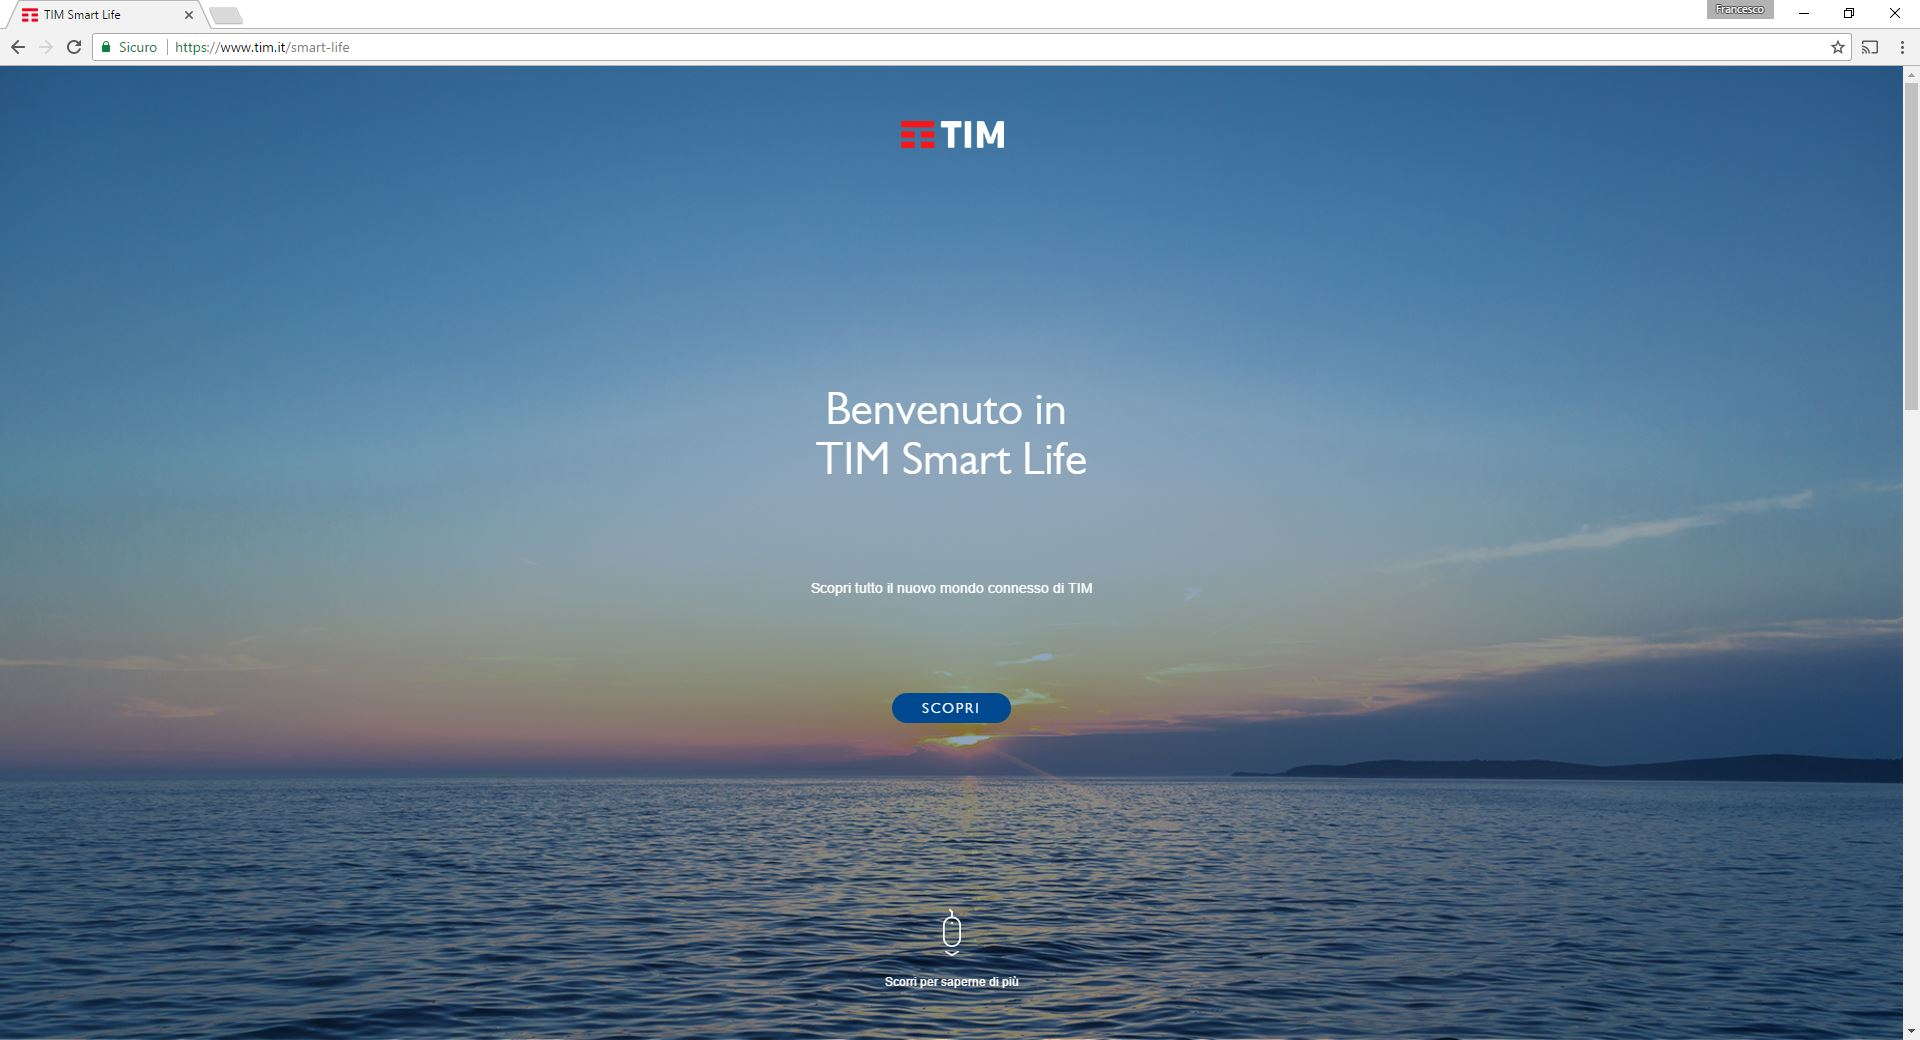
\includegraphics[width=\textwidth]{Screenshot/smartlife1.jpg}
\end{center}
\begin{center}
	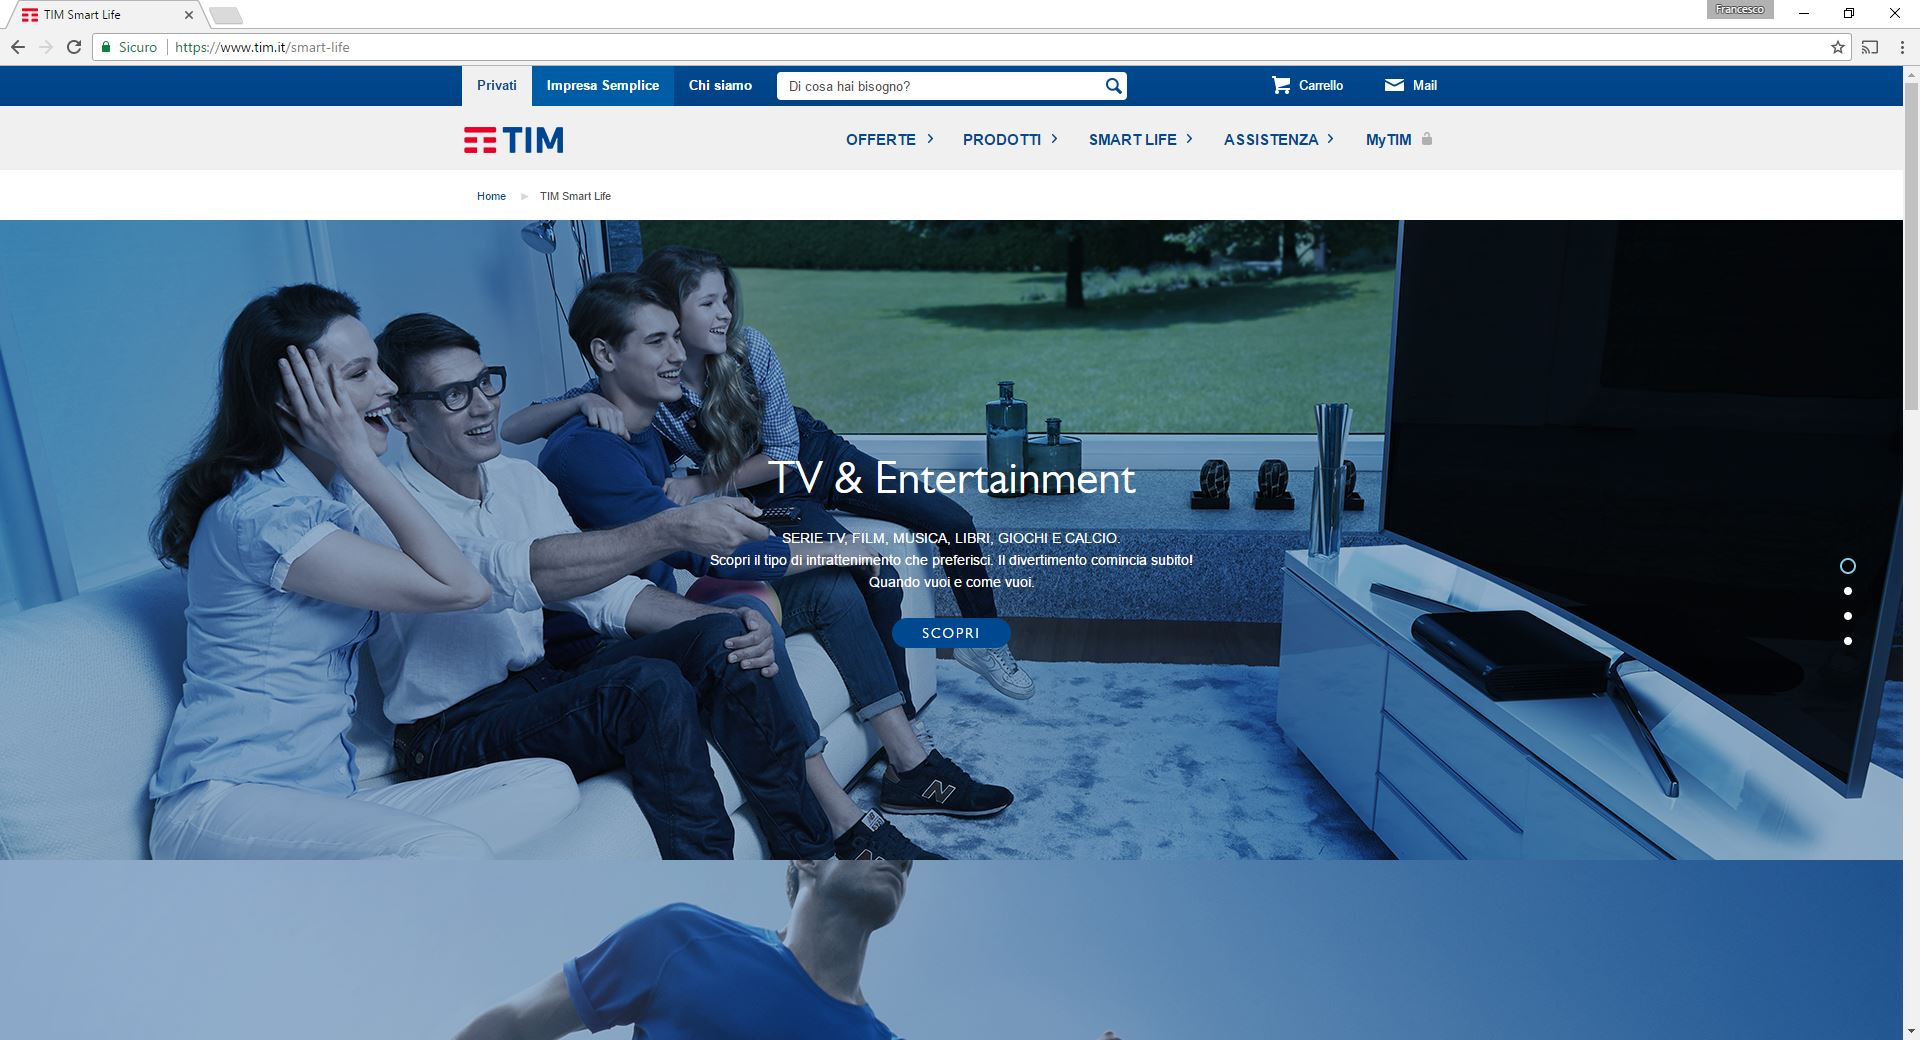
\includegraphics[width=\textwidth]{Screenshot/smartlife2.jpg}
\end{center}
\vspace{1cm}

	\paragraph*{Content heuristics \\ Text}
	\begin{itemize}
		\item accuracy: satisfied
		\item currency: \textcolor{red}{severely violated}\\
		the user cannot know if the page is updated
		\item coverage: satisfied
		\item content objectivity: satisfied
		\item authority: satisfied
		\item conciseness: satisfied		
	\end{itemize}
	
	\paragraph*{General communication quality}
	\begin{itemize}
		\item text errors: satisfied
		\item multimedia consistency: satisfied
	\end{itemize}

	\paragraph*{Navigation heuristics \\ Navigation within a topic}
	\begin{itemize}
		\item segmentation: n/a
	\end{itemize}	
	
	\paragraph*{Navigation within a transition}
	\begin{itemize}
		\item transition list: n/a
	\end{itemize}
	
	\paragraph*{Navigation within a group of topics}
	\begin{itemize}
		\item introduction list: satisfied\\
		this site identifies several groups of topics ("TV \& Entertainment", "Salute e Benessere"...)
		\item group navigation: n/a
	\end{itemize}
	
	\paragraph*{Backward navigation}
	\begin{itemize}
		\item go back: \textcolor {orange}{partially violated}\\
		there isn't a "go back" functionality but the user can exploit the TIM logo to return to the homepage or select a position in the website structure path (Home $\triangleright$ TIM Smart Life)
	\end{itemize}
	
	\paragraph*{Overall navigation}
	\begin{itemize}
		\item landmarks: satisfied\\
		they are well visible on the top-right corner of the website
		\item link consistency: satisfied
		\item orientation clues: satisfied\\
		under the logo there is a site structure path
		\item orientation clues - topic: n/a
		\item group orientation clues: n/a
		\item transition orientation clues: n/a
	\end{itemize}	
	
	\paragraph*{Visual and semantic heuristics \\ Overall graphic design }
	\begin{itemize}
		\item visual identity: satisfied
		\item chromatic code consistency: satisfied
		\item background contrast: satisfied
		\item font size: satisfied
		\item font color: satisfied
		\item font type: satisfied
		\item anchor identity: satisfied
		\item anchor states: satisfied
		\item icon consistency: satisfied
	\end{itemize}
	
	\paragraph*{Page layout}
	\begin{itemize}
		\item visual proximity: satisfied
		\item layout conventions: satisfied
		\item semiotics: satisfied
	\end{itemize}	
	
	\paragraph*{Cognitive heuristics \\ Single page}
	\begin{itemize}
		\item information overload: satisfied
	\end{itemize}	
	
	\paragraph*{Information architecture}
	\begin{itemize}
		\item classification adequacy within group of topics: n/a
		\item website mental map: satisfied
	\end{itemize}
\newpage

%------------------------------------------------------------------------------------------------------

\item Report on \url{www.tim.it/smart-life/salute-benessere}

\begin{center}
	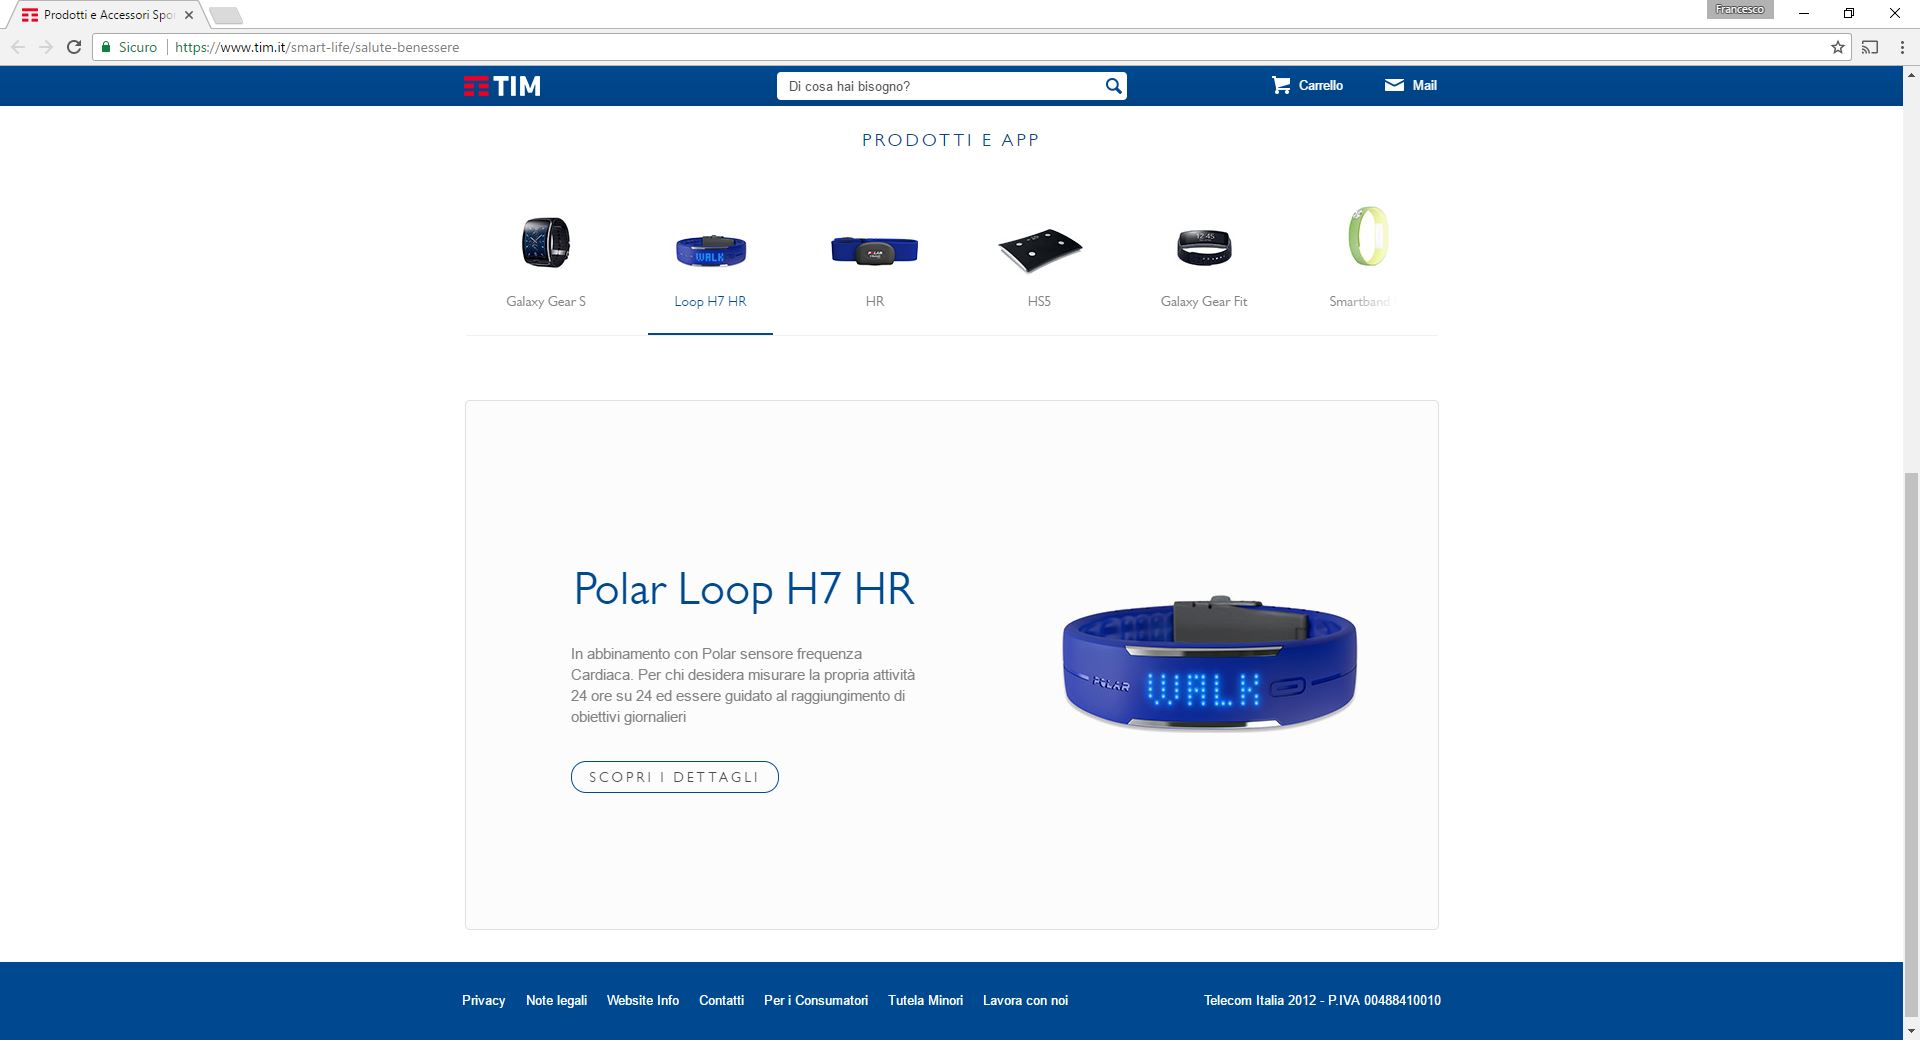
\includegraphics[width=\textwidth]{Screenshot/salute.jpg}
\end{center}
\vspace{1cm}

	\paragraph*{Content heuristics \\ Text}
	\begin{itemize}
		\item accuracy: satisfied
		\item currency: \textcolor{red}{severely violated}\\
		the user cannot know if the page is updated
		\item coverage: satisfied
		\item content objectivity: satisfied
		\item authority: satisfied
		\item conciseness: satisfied		
	\end{itemize}

	\paragraph*{General communication quality}
	\begin{itemize}
		\item text errors: satisfied
		\item multimedia consistency: satisfied
	\end{itemize}

	\paragraph*{Navigation heuristics \\ Navigation within a topic}
	\begin{itemize}
		\item segmentation: n/a
	\end{itemize}	
	
	\paragraph*{Navigation within a transition}
	\begin{itemize}
		\item transition list: n/a
	\end{itemize}
	
	\paragraph*{Navigation within a group of topics}
	\begin{itemize}
		\item introduction list: n/a
		\item group navigation: satisfied\\
		from this page it is possible to reach every item of this group of topics
	\end{itemize}

	\paragraph*{Backward navigation}
	\begin{itemize}
		\item go back: \textcolor {orange}{partially violated}\\
		there isn't a "go back" functionality but the user can exploit the TIM logo to return to the homepage or select a position in the website structure path (Home $\triangleright$ TIM Smart Life $\triangleright$ Salute e benessere)
	\end{itemize}
	
	\paragraph*{Overall navigation}
	\begin{itemize}
		\item landmarks: satisfied\\
		they are well visible on the top-right corner of the website 
		\item link consistency: satisfied
		\item orientation clues: satisfied\\
		under the logo there is a site structure path
		\item orientation clues - topic: n/a
		\item group orientation clues: satisfied
		\item transition orientation clues: n/a
	\end{itemize}	
	
	\paragraph*{Visual and semantic heuristics \\ Overall graphic design }
	\begin{itemize}
		\item visual identity: satisfied
		\item chromatic code consistency: satisfied
		\item background contrast: satisfied
		\item font size: satisfied
		\item font color: satisfied
		\item font type: satisfied
		\item anchor identity: satisfied
		\item anchor states: satisfied
		\item icon consistency: satisfied
	\end{itemize}
	
	\paragraph*{Page layout}
	\begin{itemize}
		\item visual proximity: satisfied
		\item layout conventions: satisfied
		\item semiotics: satisfied
	\end{itemize}	
	
	\paragraph*{Cognitive heuristics \\ Single page}
	\begin{itemize}
		\item information overload: satisfied
	\end{itemize}	
	
	\paragraph*{Information architecture}
	\begin{itemize}
		\item classification adequacy within group of topics: satisfied
		\item website mental map: satisfied
	\end{itemize}

%------------------------------------------------------------------------------------------------------

\item Report on \url{www.tim.it/polar-loop-activity-tracker}

\begin{center}
	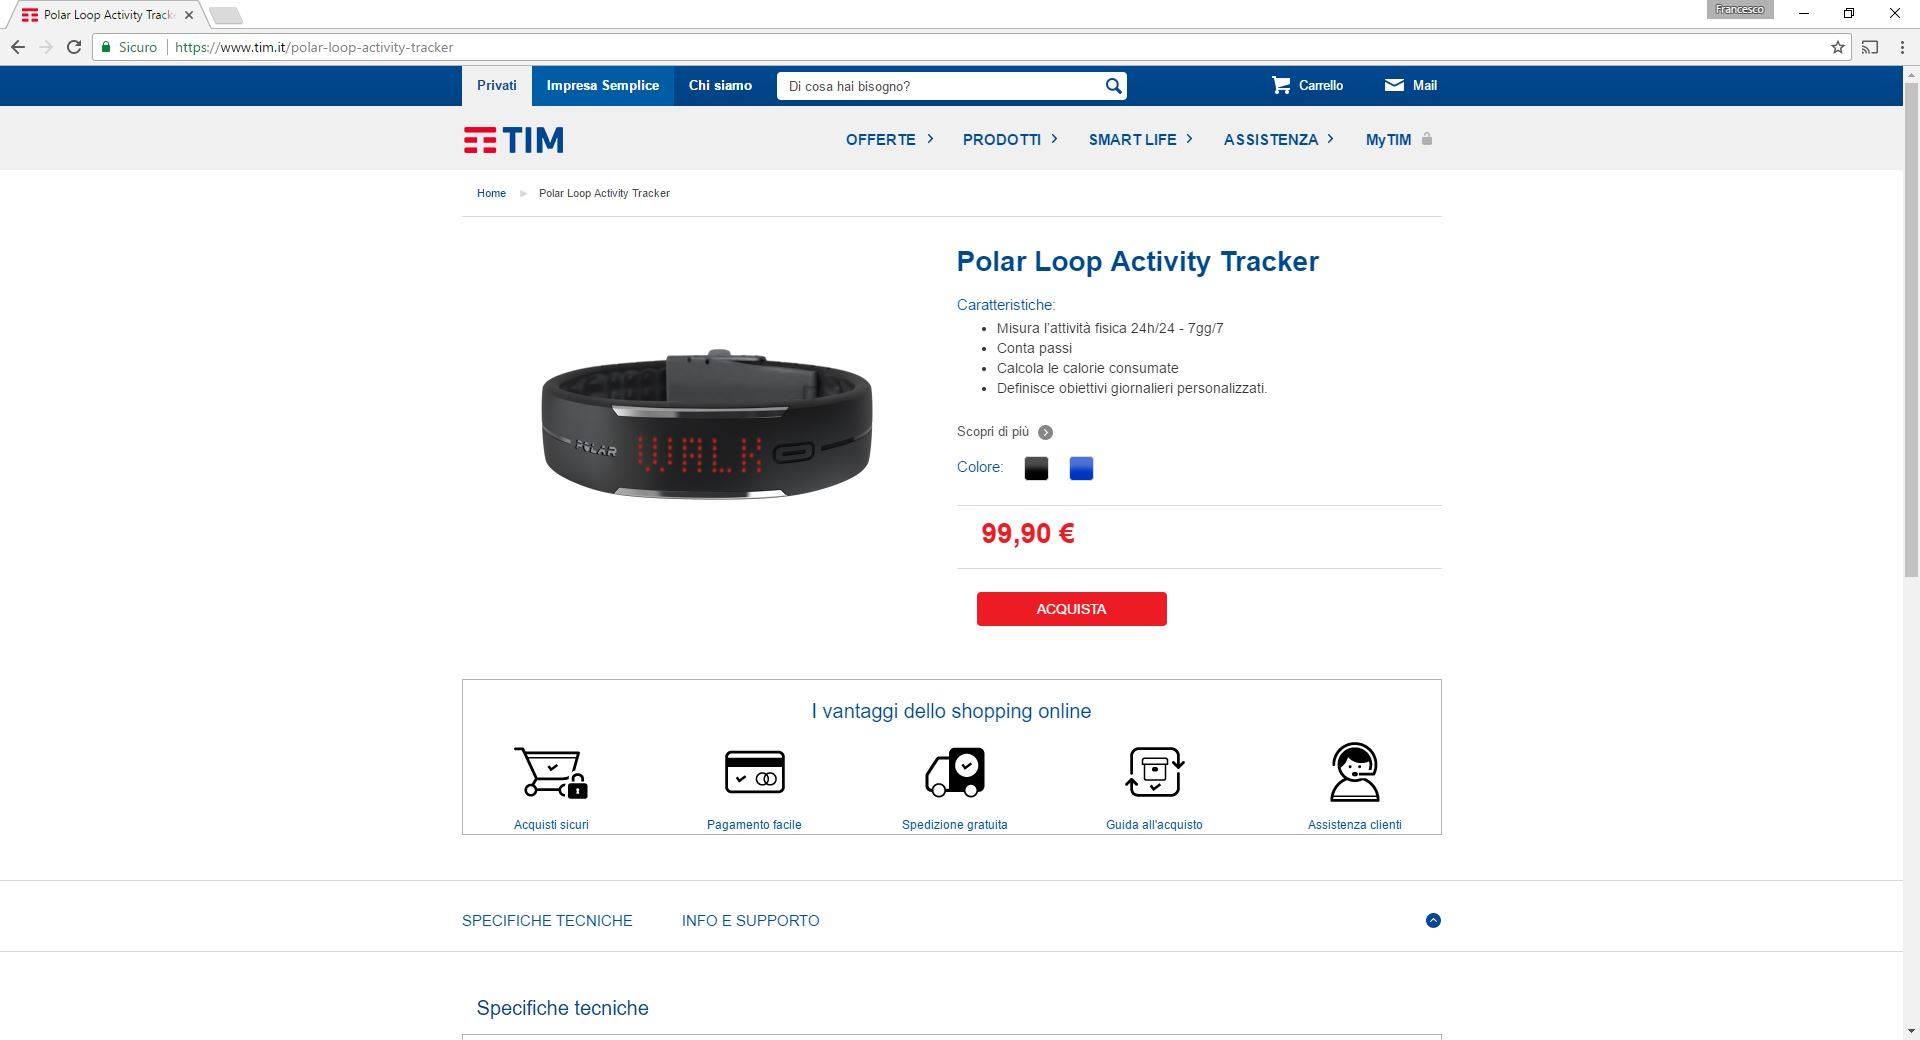
\includegraphics[width=\textwidth]{Screenshot/loop.jpg}
\end{center}
\vspace{1cm}

	\paragraph*{Content heuristics \\ Text}
	\begin{itemize}
		\item accuracy: satisfied
		\item currency: \textcolor{red}{severely violated}\\
		the user cannot know if the page is updated
		\item coverage: satisfied
		\item content objectivity: satisfied
		\item authority: satisfied
		\item conciseness: satisfied		
	\end{itemize}
	
	\paragraph*{General communication quality}
	\begin{itemize}
		\item text errors: satisfied
		\item multimedia consistency: satisfied
	\end{itemize}
	
	\paragraph*{Navigation heuristics \\ Navigation within a topic}
	\begin{itemize}
		\item segmentation: satisfied\\
		the information of the topic are organized in sub-sections on the same page 
	\end{itemize}	
	
	\paragraph*{Navigation within a transition}
	\begin{itemize}
		\item transition list: satisfied\\
		there are links related to other topics ("I vantaggi dello shopping online")
	\end{itemize}
	
	\paragraph*{Navigation within a group of topics}
	\begin{itemize}
		\item introduction list: n/a
		\item group navigation: \textcolor{red}{severely violated}\\
		the user can't reach the group by the site structure path nor items related to the group
	\end{itemize}
	
	\paragraph*{Backward navigation}
	\begin{itemize}
		\item go back: \textcolor{red}{severely violated}\\
		there is no "go back" functionality, the user can go to the homepage through the TIM logo or repeat the steps by clicking "SMART LIFE"
	\end{itemize}
	
	\paragraph*{Overall navigation}
	\begin{itemize}
		\item landmarks: satisfied\\
		they are well visible on the top-right corner of the website
		\item link consistency: satisfied
		\item orientation clues: \textcolor{orange}{partially violated}\\
		the user has a path structure that doesn't resemble his actions
		\item orientation clues - topic: satisfied\\
		the user knows the subsection he/she is visiting. When the user navigate through the site, the section's labels are well visible on top of the page
		\item group orientation clues: \textcolor{red}{severely violated}\\
		the user cannot know which group of topics he/she is visiting ("Salute e benessere")
		\item transition orientation clues: satisfied
	\end{itemize}	
	
	\paragraph*{Visual and semantic heuristics \\ Overall graphic design }
	\begin{itemize}
		\item visual identity: satisfied
		\item chromatic code consistency: satisfied
		\item background contrast: satisfied
		\item font size: satisfied
		\item font color: satisfied
		\item font type: satisfied
		\item anchor identity: satisfied
		\item anchor states: satisfied
		\item icon consistency: satisfied
	\end{itemize}
	
	\paragraph*{Page layout}
	\begin{itemize}
		\item visual proximity: satisfied
		\item layout conventions: satisfied
		\item semiotics: satisfied
	\end{itemize}	
	
	\paragraph*{Cognitive heuristics \\ Single page}
	\begin{itemize}
		\item information overload: satisfied
	\end{itemize}	

	\paragraph*{Information architecture}
	\begin{itemize}
		\item classification adequacy within group of topics: n/a
		\item website mental map: satisfied
	\end{itemize}
\newpage

%------------------------------------------------------------------------------------------------------

\item Report on \url{https://www.tim.it/prodotti/tv-e-smart-living/samsung-gear-fit}

\begin{center}
	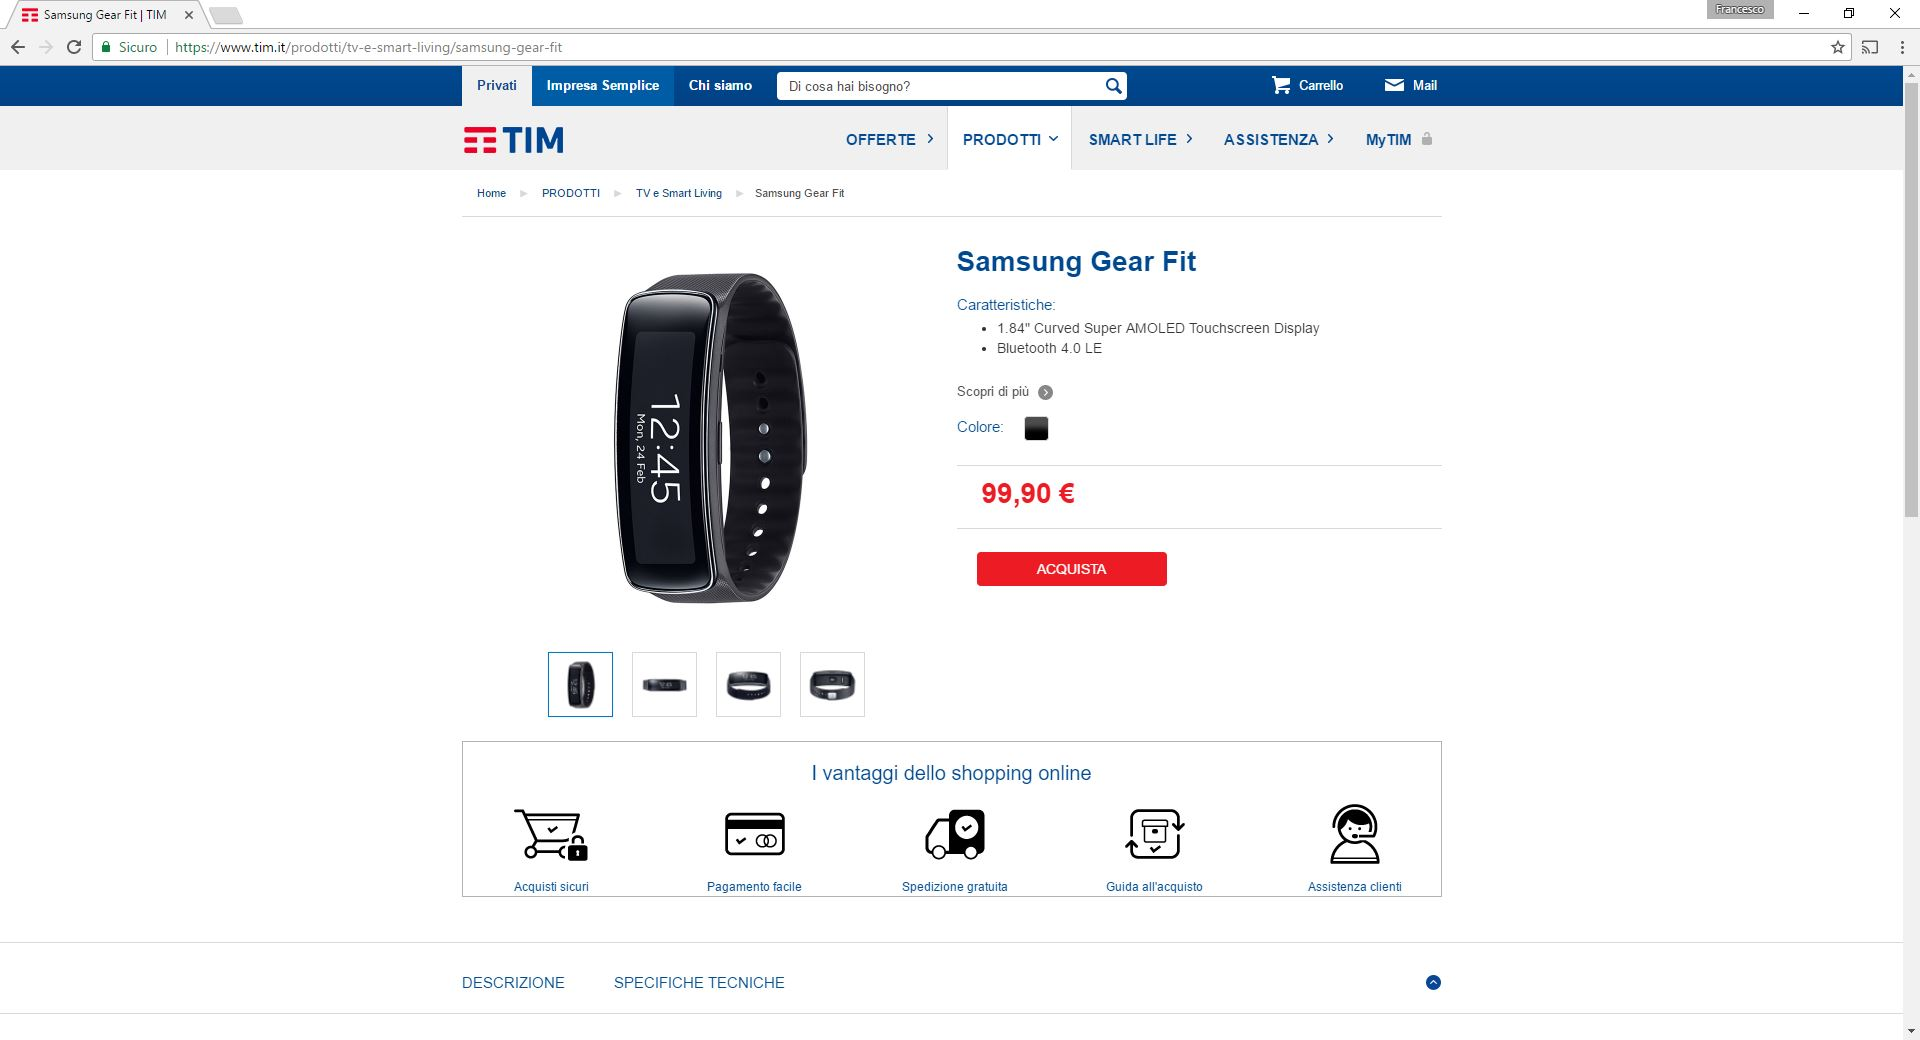
\includegraphics[width=\textwidth]{Screenshot/gear.jpg}
\end{center}
\vspace{1cm}

	\paragraph*{Content heuristics \\ Text}
	\begin{itemize}
		\item accuracy: satisfied
		\item currency: \textcolor{red}{severely violated}\\
		the user cannot know if the page is updated
		\item coverage: satisfied
		\item content objectivity: satisfied
		\item authority: satisfied
		\item conciseness: satisfied		
	\end{itemize}

	\paragraph*{General communication quality}
	\begin{itemize}
		\item text errors: satisfied
		\item multimedia consistency: satisfied
	\end{itemize}

	\paragraph*{Navigation heuristics \\ Navigation within a topic}
	\begin{itemize}
		\item segmentation: satisfied\\
		the information of the topic are organized in sub-sections on the same page
	\end{itemize}	

	\paragraph*{Navigation within a transition}
	\begin{itemize}
		\item transition list: satisfied\\
		there are links related to other topics ("I vantaggi dello shopping online")
	\end{itemize}

	\paragraph*{Navigation within a group of topics}
	\begin{itemize}
		\item introduction list: n/a
		\item group navigation: \textcolor{red}{severely violated}\\
		the user can't reach the group by the site structure path nor items related to the group
	\end{itemize}

	\paragraph*{Backward navigation}
	\begin{itemize}
		\item go back: \textcolor{red}{severely violated}\\
		there is no "go back" functionality, the user can go to the homepage through the TIM logo or repeat the steps by clicking "SMART LIFE"
	\end{itemize}

	\paragraph*{Overall navigation}
	\begin{itemize}
		\item landmarks: satisfied\\
		they are well visible on the top-right corner of the website
		\item link consistency: satisfied
		\item orientation clues: \textcolor{orange}{partially violated}\\
		the user has a path structure that doesn't resemble his actions
		\item orientation clues - topic: satisfied\\
		the user knows the subsection he/she is visiting. When the user navigate through the site, the section's labels are well visible on top of the page
		\item group orientation clues: \textcolor{red}{severely violated}\\
		the user cannot know which group of topics he/she is visiting ("Salute e benessere")
		\item transition orientation clues: satisfied
	\end{itemize}	

	\paragraph*{Visual and semantic heuristics \\ Overall graphic design }
	\begin{itemize}
		\item visual identity: satisfied
		\item chromatic code consistency: satisfied
		\item background contrast: satisfied
		\item font size: satisfied
		\item font color: satisfied
		\item font type: satisfied
		\item anchor identity: satisfied
		\item anchor states: satisfied
		\item icon consistency: satisfied
	\end{itemize}

	\paragraph*{Page layout}
	\begin{itemize}
		\item visual proximity: satisfied
		\item layout conventions: satisfied
		\item semiotics: satisfied
	\end{itemize}

	\paragraph*{Cognitive heuristics \\ Single page}
	\begin{itemize}
		\item information overload: satisfied
	\end{itemize}	

	\paragraph*{Information architecture}
	\begin{itemize}
		\item classification adequacy within group of topics: n/a
		\item website mental map: satisfied
	\end{itemize}
\end{enumerate}